\documentclass[runningheads,a4paper,11pt]{report}

%\usepackage{algorithmic}
\usepackage{algorithm} 
\usepackage{array}
\usepackage{amsmath}
\usepackage{amsfonts}
\usepackage{amssymb}
\usepackage{amsthm}
\usepackage{caption}
\usepackage{comment} 
\usepackage{epsfig} 
\usepackage{fancyhdr}
\usepackage[T1]{fontenc}
\usepackage{geometry} 
\usepackage{graphicx}
\usepackage[colorlinks]{hyperref} 
\usepackage[latin1]{inputenc}
\usepackage{multicol}
\usepackage{multirow} 
\usepackage{rotating}
\usepackage{setspace}
\usepackage{subfigure}
\usepackage{url}
\usepackage{verbatim}
\usepackage{xcolor}
\usepackage{float}
\usepackage{tabto}

\geometry{a4paper,top=3cm,left=2cm,right=2cm,bottom=3cm}

\pagestyle{fancy}
\fancyhf{}
\fancyhead[LE,RO]{Holiday Helper}
\fancyhead[RE,LO]{Team's name}
\fancyfoot[RE,LO]{MIRPR 2019-2020}
\fancyfoot[LE,RO]{\thepage}

\renewcommand{\headrulewidth}{2pt}
\renewcommand{\footrulewidth}{1pt}
\renewcommand{\headrule}{\hbox to\headwidth{%
  \color{lime}\leaders\hrule height \headrulewidth\hfill}}
\renewcommand{\footrule}{\hbox to\headwidth{%
  \color{lime}\leaders\hrule height \footrulewidth\hfill}}

\hypersetup{
pdftitle={artTitle},
pdfauthor={name},
pdfkeywords={pdf, latex, tex, ps2pdf, dvipdfm, pdflatex},
bookmarksnumbered,
pdfstartview={FitH},
urlcolor=cyan,
colorlinks=true,
linkcolor=red,
citecolor=green,
}
% \pagestyle{plain}

\setcounter{secnumdepth}{3}
\setcounter{tocdepth}{3}

\linespread{1}

% \pagestyle{myheadings}

\makeindex

\graphicspath{ {./images/} }


\begin{document}

\begin{titlepage}
\sloppy
\begin{center}
BABE\c S BOLYAI UNIVERSITY, CLUJ NAPOCA, ROM\^ ANIA

FACULTY OF MATHEMATICS AND COMPUTER SCIENCE

\vspace{6cm}

\Huge \textbf{Holiday Helper}

\vspace{1cm}

\normalsize -- MIRPR report --

\end{center}


\vspace{5cm}

\begin{flushright}
\Large{\textbf{Team members}}\\
Moisil Adriana, Informatic\u a Rom\^ an\u a, 231\\
\end{flushright}

\vspace{4cm}

\begin{center}
2019
\end{center}

\end{titlepage}

\pagenumbering{gobble}

%\begin{abstract}
%	
%	Text of abstract. Short info about: project relevance/importance, inteligent methods used for solving, data involved in the numerical experiments; conclude by the the results obtained.
%\end{abstract}


\tableofcontents

\newpage

\listoftables
\listoffigures
\listofalgorithms

\newpage

\setstretch{1.5}



\newpage

\pagenumbering{arabic}


 


\chapter{Introduction}
\label{chapter:introduction}

\section{What? Why? How?}
\label{section:what}

Motivate and abstractly describe the problem you are addressing and how you are addressing it. 
\begin{itemize}
	\item What is the (scientific) problem? 
	\newline
	The problem tackles natural language processing, natural language understanding and image classification. The user is going to describe in natural language the basic requirements for their vacation: location, number of rooms, number of kids, dates, or they can provide an image to substitute for a location (and based on it, the AI algorithm will deduce which type of destination is most suitable for them).
	\item Why is it important? 
	\newline
	It is a holiday helper assistant, meaning that it will help the users with a general idea of their vacation needs to make a first impression of the available accommodation options.
	\item What is your basic approach? 
	\newline
	We are building a prototype demonstrating the basic functionalities of the app. This includes recognizing a few filters from the user input, and using the Booking API together with our AI algorithm to give hotel recommendations.
\end{itemize}


\chapter{Scientific Problem}
\label{section:scientificProblem}

\section{Open text analysis}
\label{section:openTextAnalysis}
The first part of the application's flow is extracting the user's requirements from open text. Giving a friendlier experience is the motivation behind building it as a chatbot, so that's why we decided to allow this type of input. We're using the nltk and spacy libraries in order to extract all the information we need:
\begin{itemize}
	\item location
	\item time period
	\item number of rooms
	\item number of children
\end{itemize}  

\subsection{Extract number of rooms}
For extracting the number of rooms, we build a custom grammar (called COUNT) that is used when parsing the input (using nltk.nltkRegexpParser):
\newline
COUNT:\{
\newline\tab<CD><NNS>|
\newline\tab<CD><JJ>*<NNS>|
\newline\tab<CD>(<JJ><CC>)*<JJ><NNS>|
\newline\tab<CD><NN>|
\newline\tab<CD><JJ>*<NN>|
\newline\tab<CD>(<JJ><CC>)*<JJ><NN>
\newline\}
\newline
The custom grammar can recognize all the groups that start with a cardinal, end with a noun (both singular and plural) and might contain adjectives and conjunctions in between (e.g. 'two spacious and bright rooms'). 

\begin{figure}[H]
	\caption{Extract number of rooms.}
	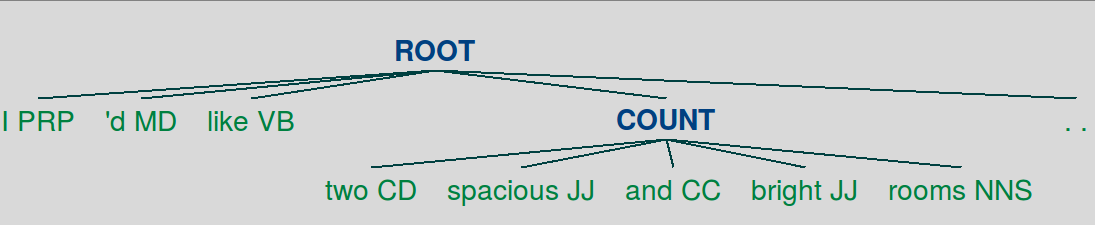
\includegraphics[trim={0 0 0 1cm},clip,width=15cm]{extract_rooms.png}
	\centering
\end{figure}

\subsection{Extract number of children}
We tried implementing a different approach for extracting the number of children. We make use of the tokens' dependencies in order to find the cardinal that is associated with the noun children (or similar nouns).

\begin{figure}[H]
	\caption{Extract number of children.}
	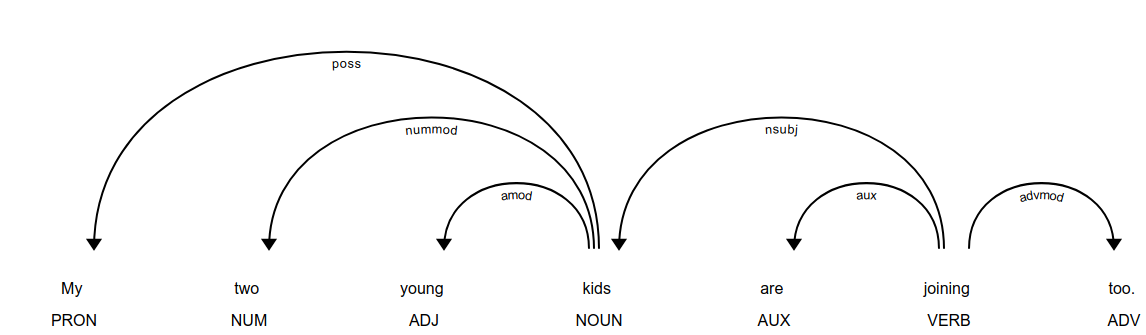
\includegraphics[trim={0 0 0 1cm},clip,width=15cm]{extract_children.png}
	\centering
\end{figure}


\section{Image classifier}
\label{section:imageClassifier}
We built an image classifier using Keras, which is TensorFlow's high-level API for building and training deep learning models. The user can upload an image (for demonstration purposes only, the current input images are limited to forests, sand beaches and snow mountains) to which the application will offer suggestion of destinations that look similar to what the user wants. The image will be rejected and the application will ask the user again for their desired location (either through an another image or through text) if the probability for the image to fit in one of the three categories is too low.


\begin{table}[H]
	\caption{The parameters used for training the Keras model used for image classification.}
	\begin{center}
		\begin{tabular}{p{220pt}c}
			\textbf{Parameter}& \textbf{Value} \\
			\hline\hline
			Batch size & 64 \\
			Number of epochs & 10 \\
			Image height & 150 \\
			Image width & 150 \\
			Learning rate & 0.0001 \\
		\end{tabular}
	\end{center}
\end{table}


\begin{table}[H]
	\caption{The layers of the Keras model used for image classification.}
	\begin{center}
		\begin{tabular}{p{120pt}p{150pt}p{70pt}}
			\textbf{Layer type} & \textbf{Output Shape} & \textbf{Param \#} \\
			\hline\hline
			Conv2D & (None, 150, 150, 16) & 448 \\
			MaxPooling2D & (None, 75, 75, 16) & 0 \\
			Conv2D & (None, 75, 75, 32) & 4640 \\
			MaxPooling2D & (None, 37, 37, 32) & 0 \\
			Conv2D & (None, 37, 37, 64) & 18496 \\
			MaxPooling2D & (None, 18, 18, 64) & 0 \\
			Dropout & (None, 18, 18, 64) & 0 \\
			Flatten & (None, 20736) & 0 \\
			Dense & (None, 512) & 10617344 \\
			Dense & (None, 3) & 1539 \\
		\end{tabular}
	\end{center}
\end{table}
		
\begin{figure}[H]
	\caption{Training and Validation values for the final model.}
	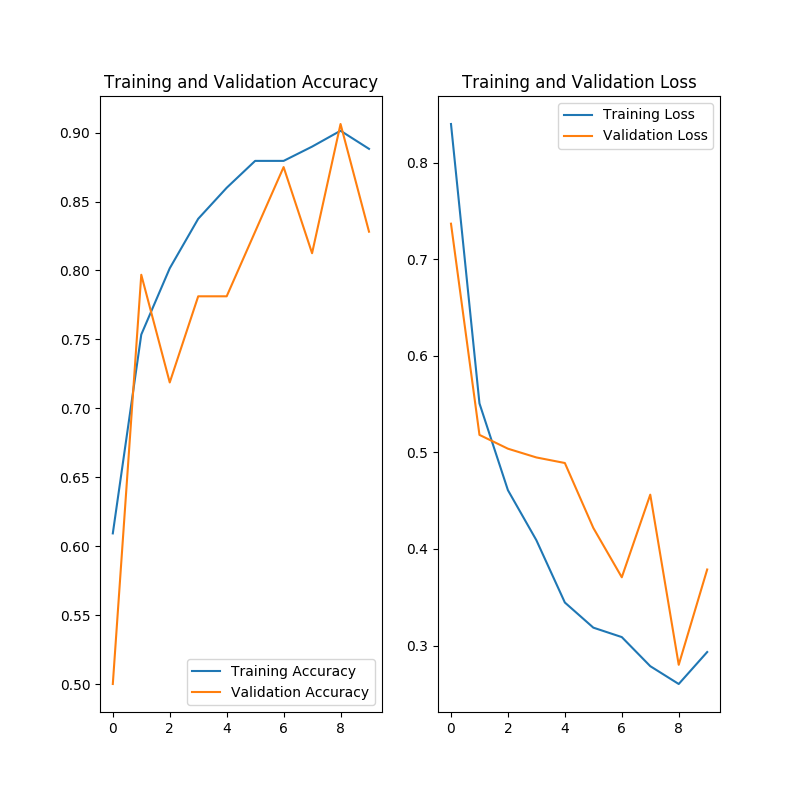
\includegraphics[trim={0 0 0 1cm},clip,width=15cm]{training_and_validation.png}
	\centering
\end{figure}


\section{Reviews analyzer}
Apart from the Image Classifier, the tool contains what we call a "Reviews analyzer". Given the raw user reviews extracted from Booking (both the negative and the positive ones), it does the following:
\begin{itemize}
	\item Clusters data and extracts the topics for each cluster
	\begin{itemize}
		\item Preprocesses the raw text (remove stopwords, punctuation, spelling correction etc.; no stemmer or lemmatizer is being used here)
		\item Encodes the data using Tensorflow's Universal Sentence Encoder, which, for each input text, returns an array of 512 floating points
		\item Clusters the data using the clustering algorithms implementations offered by the scikit-learn and hdbscan libraries. The clustering methods that were tested are KMeans, DBSCAN, HDBSCAN and Agglomerative, and based on the results, we moved forward with the last one.
		\item Extract the keywords for each cluster (Bag of Words)
	\end{itemize}
	\item Creates word clouds (the preprocessing of the raw text in this case is different as the words are lemmatized WordNetLemmatizer from the nltk library)
	\item Computes the overall sentiment (a value between -1 and 1, -1 representing a negative sentiment and 1 representing a positive one) for each hotel (using the textblob library)
\end{itemize}

		
\chapter{State of art/Relate work}
\label{chapter:stateOfArt}
\section*{Google Assistant}
\begin{itemize}
	\item Virtual Assistant (not for travel planning)
	\item Stand alone app
\end{itemize} 

\section*{Hello Hipmunk}
\begin{itemize}
	\item Virtual Travel planning assistant
	\item Integrated with Facebook Messenger, Slack, Skype
	\item Available to group chats
	\item Includes flights and hotels
	\item Deals only with traveling (doesn't help with dinner or entertainment)
\end{itemize}

\section*{Mezi}
\begin{itemize}
	\item Stand alone app
	\item Includes flights, hotels and restaurant reservations	
	\item Provides interactive output (buttons to book a flight)
\end{itemize}

\section*{SnapTravel}
\begin{itemize}
\item Virtual Travel Planning Assistant
\item Integrated with Facebook Messenger and Whatsapp
\end{itemize}

\section*{HelloGBye}
\begin{itemize}
\item Virtual Travel Planning Assistant
\item Text and voice recognition	
\item Provides interactive output (buttons to book a flight)
\end{itemize}

\section*{Holiday Helper}
\begin{itemize}
	\item Stand alone app
	\item Includes only hotels, using the Booking API
	\item The information is asked for in multiple rounds, not all at once, unless the user provides more (e.g. both the location, number of people and number of rooms) at a time.
	\item Text recognition only
\end{itemize}

\begin{table}[h]
	\centering
	\begin{tabular}{|c|c|c|c|c|c|}
		\hline
		& Hello Hipmunk & Mezi & SnapTravel & HelloGBye & Holiday Helper \\ \hline
		Stand alone app & NO & YES & YES & YES & YES \\ \hline
		Messenger & YES & NO & {\color[HTML]{333333} YES} &  NO & NO \\ \hline
		Whatsapp & NO & NO & YES & NO & NO \\ \hline
		Slack & YES & NO & NO & NO & NO \\ \hline
		Skype & YES & NO & NO & NO & NO \\ \hline
		Hotels & YES & YES & YES & YES & YES \\ \hline
		Restaurants & NO & YES & NO & NO & NO \\ \hline
		Flights & YES & YES & YES & YES & NO \\ \hline
	\end{tabular}
\end{table}


\chapter{Proposed approach}
\label{chapter:proposedApproach}

We're using a client-server model for this solution in order to make it portable. When it comes to the technologies we used, the backend is a Flask server while the frontend is built using Django. All the logic takes place on the server, so the client only sends the data to it and waits for the results. As a result, the application can run on any device (computer, smartphone), as long as it's connected to the Internet (and the server is running).


\chapter{Application (numerical validation)}
\label{chapter:application}


Explain the experimental methodology and the numerical results obtained with your approach and the state of art approache(s).

Try to perform a comparison of several approaches.

Statistical validation of the results.


\section{Methodology}
\label{section:methodology}

\begin{itemize}
	\item What are criteria you are using to evaluate your method? 
	\item What specific hypotheses does your experiment test? Describe the experimental methodology that you used. 
	\item What are the dependent and independent variables? 
	\item What is the training/test data that was used, and why is it realistic or interesting? Exactly what performance data did you collect and how are you presenting and analyzing it? Comparisons to competing methods that address the same problem are particularly useful.
\end{itemize}

\section{Data}
\label{section:data}

\subsection{Image classifier}
The data used for training the Image Classifier was collected from Google Images using a script, obtaining around 800 entries for each section (forest, sand beach and snow mountain). After filtering, the remaining number is around 450 for the first two categories, and 680 for the last one, which were later divided in two sections: training and validation. In total, there were used 1496 images for training and 150 for validation. 

\section{Results}
\label{section:results}

One way to improve the results of our model used for image classification would consist of gathering more training data for all the three existing categories.


\chapter{Conclusion and future work}
\label{chapter:concl}

\section{Open text analysis}

\section{Image classifier}
Our current dataset for training and validation is quite small, so one way to improve this component is gathering more images for the three categories in order to train the model better. It would be also worth looking into ways of adjusting the ImageDataGenerator's parameters for the training and validation images so we can generate more data from the current one.

\section{Reviews analyzer}
As mentioned before, we consider the cluster's keywords to be their most frequent words. This might not always lead to the best result (e.g. a cluster with positive reviews where the main topic is breakfast, but we don't know what other words are associated with it: it could be 'large breakfast' or 'delicious breakfast' etc.), so another option would be extracting pairs of two words as keywords.

%\bibliographystyle{plain}
%\bibliography{BibAll}

\end{document}